\documentclass[11pt]{article}
% Shared preamble for the report (XeLaTeX). Fonts ship with TeX Live / MacTeX.
\usepackage[letterpaper,margin=1in,headsep=0.3in,footskip=0.4in]{geometry}
\usepackage{fontspec}
\usepackage{unicode-math}
\setmainfont{TeX Gyre Termes}
\setsansfont{TeX Gyre Heros}[Scale=MatchLowercase]
\setmonofont{DejaVu Sans Mono}[Scale=0.82]
\setmathfont{TeX Gyre Termes Math}
\usepackage{microtype}
\linespread{1.0}
\emergencystretch=1.5em
\setlength{\parindent}{1.4em}
\setlength{\parskip}{0pt}
\frenchspacing
\widowpenalty=10000 \clubpenalty=10000

% colours
\usepackage{xcolor}
\definecolor{linkblue}{HTML}{1A4F8B}
\definecolor{muted}{HTML}{5B6270}
\definecolor{rule}{HTML}{9AA1AC}

% headings: numbered, bold, as in HW5
\usepackage{titlesec}
\titleformat{\section}{\normalfont\fontsize{12}{14}\bfseries}{\thesection.}{0.5em}{}
\titleformat{\subsection}{\normalfont\normalsize\bfseries}{\thesubsection}{0.6em}{}
\titleformat{\subsubsection}[runin]{\normalfont\normalsize\bfseries}{}{0em}{}[.]
\titlespacing*{\section}{0pt}{14pt plus 3pt minus 2pt}{6pt plus 1pt}
\titlespacing*{\subsection}{0pt}{10pt plus 2pt minus 2pt}{4pt plus 1pt}
\titlespacing*{\subsubsection}{0pt}{6pt plus 2pt}{0.6em}
\newcommand{\para}[1]{\par\smallskip\noindent\textbf{#1}\hspace{0.5em}}

% lists
\usepackage{enumitem}
\setlist{itemsep=2pt,parsep=0pt,topsep=4pt,leftmargin=1.6em}

% tables and figures
\usepackage{booktabs,threeparttable,makecell,multirow,array,tabularx}
\renewcommand{\arraystretch}{1.12}
\setlength{\aboverulesep}{0.3ex}\setlength{\belowrulesep}{0.5ex}
\usepackage{graphicx}
\usepackage{flafter}  % floats never precede their first mention
\usepackage[labelfont=bf,labelsep=period,font=small,justification=justified,
            singlelinecheck=false,skip=5pt]{caption}
\captionsetup[table]{position=top}
\renewcommand{\TPTnoteSettings}{\setlength\leftmargin{0pt}\setlength\labelwidth{0pt}\setlength\labelsep{0pt}\setlength\itemsep{1pt}}
\setlength{\textfloatsep}{14pt plus 3pt minus 3pt}
\setlength{\floatsep}{12pt plus 3pt minus 3pt}
\renewcommand{\topfraction}{0.9}\renewcommand{\bottomfraction}{0.6}
\renewcommand{\textfraction}{0.1}\renewcommand{\floatpagefraction}{0.8}

% running head and page numbers
\usepackage{fancyhdr}
\pagestyle{fancy}
\fancyhf{}
\renewcommand{\headrulewidth}{0pt}
\fancyhead[R]{\footnotesize\color{muted}\shorttitle}
\fancyfoot[C]{\small\thepage}
\fancypagestyle{plain}{\fancyhf{}\renewcommand{\headrulewidth}{0pt}\fancyfoot[C]{\small\thepage}}

% references and links
\usepackage[numbers,square,sort&compress]{natbib}
\setlength{\bibsep}{2pt plus 1pt}
\renewcommand{\bibfont}{\small}
\usepackage[colorlinks=true,linkcolor=linkblue,citecolor=linkblue,urlcolor=linkblue]{hyperref}
\usepackage[nameinlink,capitalise,noabbrev]{cleveref}
\crefname{table}{Table}{Tables}
\crefname{figure}{Figure}{Figures}

% title block
\newcommand{\shorttitle}{}
\newcommand{\papertitle}[1]{\def\@ptitle{#1}}
\makeatletter
\newcommand{\maketitleblock}[4]{% title, author line, info line, abstract
  \thispagestyle{plain}
  \begin{center}
    {\fontsize{16.5}{20}\selectfont\bfseries #1\par}
    \vspace{9pt}
    {\normalsize #2\par}
    \vspace{2pt}
    {\small\color{muted}#3\par}
  \end{center}
  \vspace{4pt}
  \begin{center}\textbf{Abstract}\end{center}
  \vspace{-4pt}
  {\small\leftskip=0.45in\rightskip=0.45in\noindent #4\par}
}
\makeatother
\newcommand{\keywords}[2]{%
  \vspace{5pt}
  {\small\leftskip=0.45in\rightskip=0.45in\noindent\textit{Keywords:} #1\par
   \noindent\textit{JEL codes:} #2\par}
  \vspace{6pt}{\centering\color{rule}\rule{0.35\textwidth}{0.4pt}\par}\vspace{2pt}}

\renewcommand{\shorttitle}{Unexplained Pessimism Ahead of the 2026 Midterms}
\begin{document}

\maketitleblock
{Unexplained Pessimism:\\Economic Fundamentals, Media Narratives, and\\U.S.\ Consumer Sentiment Ahead of the 2026 Midterms}
{Jonas Wu (jw9452)}
{AI Applications in Finance, Final Project\\Data cutoff: October 16, 2026 \quad·\quad Replication package: \textit{link to be added}}
{U.S. consumer sentiment has stayed far below the level implied by headline economic indicators. Using the real-time vintages of unemployment, PCE inflation and real GDP growth that were available at each survey date, we fit an economic-only model to the University of Michigan Index of Consumer Sentiment over 2010–2019 and define the sentiment gap as its out-of-sample residual. The gap averages −35.8 index points in 2025 and −39.8 in January–October 2026, and the three indicators account for only 7–11\% of the decline since 2019. To ask whether news and social media help explain the gap, we code a documented corpus with a large language model validated against 360 items labeled independently by two human annotators (tone $\kappa = 0.73$, against 0.79 between the annotators and 0.35 for a finance dictionary). Swapping political names does not detectably change the coding. Lagged national news tone improves forecasts over the economic-only model (Clark–West $p = 0.041$) but not once household-pressure and political controls are added ($p = 0.23$; none of 20 variants significant), and tone-related variation accounts for at most about 5\% of the 2025–2026 gap. The gap is similar across income, age, region and education groups, widens within the web-only survey period, and is present before the campaign season. Media bias is therefore not the main explanation of the gap; we propose a randomized framing experiment for causal identification.}
\keywords{consumer sentiment; real-time data; media bias; large language models; forecasting; 2026 midterm elections}{D12, D84, E71, C53}

\section{Introduction}

Since mid-2021, U.S. consumers have reported far gloomier views of the economy than unemployment, inflation and output growth would suggest. Such a gap invites three different readings. Consumers may be responding to pressures that headline indicators miss, such as the level of prices or the cost of housing. Their perceptions may instead reflect selective information, framing or cognitive bias, possibly transmitted through news and social media. Or the apparent discrepancy may be an artifact of measurement, timing or an incomplete model. This paper treats all three as hypotheses (H1–H3) and asks which the available evidence can support or rule out ahead of the November 3, 2026 midterm elections.

We make three contributions, each registered before the results were computed:
\begin{itemize}
  \item \textbf{A real-time baseline.} Every indicator enters at the vintage published before the survey month, so the gap measures pessimism relative to information consumers could actually have had (\cref{sec:baseline}).
  \item \textbf{Validated AI measurement.} An LLM codes tone, salience, framing, factual calibration and political attribution against a human gold standard, with a dictionary and a conventional classifier as benchmarks.
  \item \textbf{Separate tests of association and causation.} Chronological forecast comparisons, timing tests and pre-registered falsification criteria are reported together with a design for stronger identification.
\end{itemize}

\section{Data and the real-time economic baseline}\label{sec:baseline}

\subsection{Real-time indicators}
For each survey month $t$ we take the U-3 unemployment rate, year-over-year headline PCE inflation and real GDP growth from the ALFRED vintage available on the first day of $t$ \citep{croushore2001}. GDP growth is the latest published quarter-over-quarter annualized rate and is held constant between releases rather than interpolated. The economic-only model (M1) is
\begin{equation}
  \mathit{ICS}_t = \alpha + \beta_u U^{\mathrm{rt}}_t + \beta_\pi \pi^{\mathrm{rt}}_t + \beta_g g^{\mathrm{rt}}_t + \textstyle\sum_{m} \delta_m D_{mt} + \varepsilon_t ,
  \label{eq:m1}
\end{equation}
estimated on 2010–2019 with HAC standard errors; the sentiment gap is $\mathit{ICS}_t - \widehat{\mathit{ICS}}_t$ for every month after 2019. A negative gap is unexplained pessimism under M1, not evidence of perceptual bias.

\subsection{The size of the gap}
M1 fits the estimation window closely ($R^2 = 0.90$; unemployment $-4.84$, s.e.\ 0.29). \Cref{fig:gap} shows that a large and growing gap opens from the second half of 2021, and \cref{tab:gap} summarizes it by period. The 2025 and 2026 gaps are roughly eight times the half-width of the M1 prediction band, and the current-conditions component (ICC) is consistently further below its prediction than the expectations component (ICE).

\begin{table}[htbp]
\centering
\begin{threeparttable}
\caption{\textbf{Sentiment gap relative to the economic-only model (M1), by period}}
\label{tab:gap}
\small
\begin{tabular}{@{}l r r r c r r r@{}}
\toprule
 & & \multicolumn{4}{c}{Index of Consumer Sentiment (ICS)} & \multicolumn{2}{c}{Mean gap}\\
\cmidrule(lr){3-6}\cmidrule(l){7-8}
Period & Months & \makecell[r]{Actual\\change} & \makecell[r]{Mean\\gap} & \makecell{95\% band\\under M1} & \makecell[r]{Explained\\share $S$} & ICC & ICE\\
\midrule
2021-07 to 2022-12 & 18 & −32.6 & −22.9 & [−7.7, 7.9] & 0.30 & −35.0 & −15.2 \\
2023-01 to 2024-12 & 24 & −27.0 & −25.2 & [−4.4, 4.7] & 0.07 & −39.8 & −15.8 \\
2025-01 to 2025-12 & 12 & −38.4 & −35.8 & [−4.2, 3.9] & 0.07 & −47.7 & −28.2 \\
2026-01 to 2026-10 & 10 & −44.8 & −39.8 & [−5.3, 5.1] & 0.11 & −55.2 & −29.9 \\
\bottomrule
\end{tabular}
\begin{tablenotes}[flushleft]\footnotesize
\item \textit{Notes:} Changes are relative to the 2019 average. Gap = actual − M1 out-of-sample prediction; M1 regresses each index on real-time U-3 unemployment, PCE inflation (year over year) and real GDP growth (quarter over quarter, annualized), fitted on 2010–2019 with month dummies. The band is the 95\% range of the period-mean prediction error under M1 (moving-block bootstrap, block length 12, 2,000 draws); every period mean lies outside it ($p < 0.001$). $S = 1 - \text{mean gap}/\text{actual change}$, the share of the decline since 2019 that M1 accounts for. ICC = Current Economic Conditions; ICE = Consumer Expectations. Pandemic months (2020-01 to 2021-06) are omitted. 2026-10 is the preliminary reading.
\item \textit{Source:} \texttt{results/stage1\_m1/m1\_periods.csv}.
\end{tablenotes}
\end{threeparttable}
\end{table}


\begin{figure}[htbp]
  \centering
  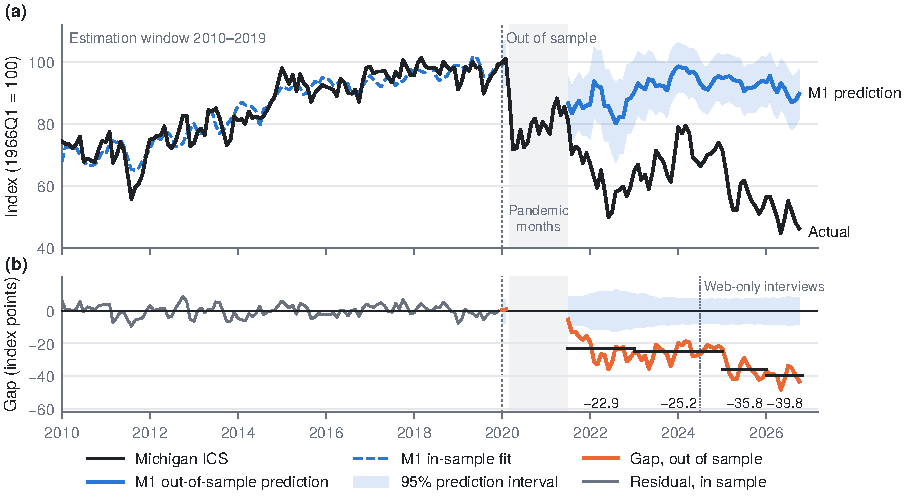
\includegraphics[width=\textwidth]{figures/fig_gap.pdf}
  \caption{\textbf{Michigan sentiment against the economic-only prediction.} Panel (a) shows the Index of Consumer Sentiment and the M1 prediction from \cref{eq:m1}; the dashed line is the 2010–2019 in-sample fit and the band is the 95\% moving-block bootstrap prediction interval. Panel (b) shows the gap; horizontal segments and labels give the period means in \cref{tab:gap}. Pandemic months (shaded) are not interpreted because the indicators leave the estimation range. The dotted line marks the first month of web-only interviewing (July 2024).}
  \label{fig:gap}
\end{figure}

\para{What the gap is not.} The specimen ends here. In the full report this subsection continues with the alternative explanations (household pressure, survey mode, partisan composition) and the forecast comparison uses the test of \citet{clark2007}; local projections follow \citet{jorda2005}, and the dictionary benchmarks follow \citet{loughran2011} and \citet{shapiro2022}.

\bibliographystyle{unsrtnat}
\bibliography{references}

\end{document}
